\subsection{Conservação do Momento Angular}
Nessa parte do relatório, temos três subitens:

No primeiro deles, iremos tratar de uma análise do movimento de atletas e a sua relação com a conservação do momento angular. Dessa forma, usaremos vídeos e imagens dos esportistas em suas práticas e fim de entender a parte física das execuções, principalmente fazendo relação de suas rotações (ora mais rápidas ora mais lentas) com os conceitos de conservação de momento angular, utilizando a fórmula:

\[I_1 \omega _1 = I_2 \omega _2 \]

Na segunda parte, falaremos do experimento do banquinho giratório. Para realizá-lo, utilizaremos um banco - que pode girar praticamente sem atrito ao redor de um eixo vertical. Um colaborador vai sentar nesse banco, segurando dois halteres (de massa qualquer), inicialmente, com os braços abertos. Alguém irá impulsionar a pessoa sentada, que começará a girar com pequena velocidade angular. Em um dado instante, o colaborador irá fechar os braços, aproximando os halteres do peito e, por conta da conservação de momento angular, sua velocidade angular irá aumentar, como demonstrado pela fórmula:

\[I_1 \omega _1 = I_2 \omega _2 \]

Por fim, trataremos do experimento do banco giratório com a roda de bicicleta, que consiste num banco sem atrito - semelhante ao do tópico anterior - e uma roda de bicicleta presa a um eixo. Inicialmente, o colaborador senta-se no banco e segura a roda da bicicleta com o eixo na vertical - não havendo torques na direção vertical do sistema banco-colaborador-roda, havendo uma conservação da quantidade de movimento angular nesse eixo vertical. Coloca-se a roda em movimento, em torno de seu eixo com certa velocidade angular, mas o banco e o colaborador estão em repouso.

Algum tempo depois, inclina-se o eixo de rotação da roda a um ângulo $\phi$, em relação à horizontal - como mostra a figura 5. Assim, surge uma componente de momento angular na direção vertical, por conta da rotação da roda. Como o momento angular é constante na direção vertical - que é nulo nesse caso - é necessário que apareça outra componente de momento que anule a componente vertical criada pela inclinação da roda. Assim, essa nova componente surgirá e fará o banco rodar junto com a pessoa, no sentido contrário ao sentido de rotação da roda de bicicleta.

\begin{figure}[H]
  \centering
  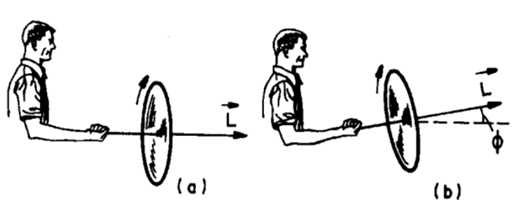
\includegraphics[scale=1]{images/i5.png}
  \caption{Roda de Bicicleta Giratória}
\end{figure}
